% ============================================================
%  DLCO 实验报告模板（lab02 实例）
%  【复用】复制整个 report/ 到 labNN/report/，改 \expname、\expdate + TODO 处 + 换 figures/ 图片
%  【编译】整个 lab 目录上传 tex.nju.edu.cn，编译 main.tex，下载 main.pdf 放回本目录
%  【提交】工程文件 + 报告电子版打包 zip 上传
%
%  lab02 图占位约定（截图后存到 figures/，取消对应 figure 环境的注释）：
%    figures/lab02_build.png  实验过程：Vivado 综合/实现成功（build.bat 输出）
%    figures/lab02_wave.png   实验结果-仿真：Vivado 波形图（建议截 A/B/ALUctr/F/cf/zero/of）
%    figures/lab02_board.jpg  实验结果-上板：开发板实测照片（可选）
% ============================================================
\documentclass[12pt, a4paper]{ctexart}

\usepackage{geometry}
\geometry{left=2.5cm, right=2.5cm, top=3cm, bottom=3cm}
\usepackage{listings}
\usepackage{graphicx}
\usepackage{xcolor}
\usepackage{amsmath}
\usepackage{tikz}

\graphicspath{{figures/}}

% ---------------- 代码高亮设置 ----------------
\lstset{
    language=Verilog,
    basicstyle=\ttfamily\small,
    frame=single,
    framesep=5pt,
    numbers=left,
    numberstyle=\tiny\color{gray},
    keywordstyle=\color{blue},
    commentstyle=\color{gray},
    breaklines=true,
    showstringspaces=false,
    tabsize=4
}

% ---------------- 封面信息（复用改 \expname、\expdate） ----------------
\newcommand{\coursename}{数字逻辑与计算机组成实验}
\newcommand{\expname}{lab02：简易 ALU 运算器}
\newcommand{\expdate}{2026-09-06}
\newcommand{\stuname}{法童}
\newcommand{\stuid}{251250046}
\newcommand{\stumail}{251250046@smail.nju.edu.cn}

\begin{document}

% 封面
\begin{titlepage}
    \centering
    \vspace*{4cm}
    {\Huge\bfseries 实验报告\par}
    \vspace{1.5cm}
    {\Large \coursename\par}
    \vspace{0.8cm}
    {\Large \expname\par}
    \vspace{3cm}
    {\large
    \begin{tabular}{rl}
        姓名： & \stuname \\
        学号： & \stuid \\
        邮箱： & \stumail \\
        实验时间： & \expdate \\
    \end{tabular}\par}
\end{titlepage}

\section{实验目的}
\begin{enumerate}
    \item 掌握用行为级 Verilog 描述 4 位简易 ALU，通过 3 位功能选择端 \texttt{ALUctr}（\texttt{casez}）完成加、减、按位取反、与、或、异或、有符号小于比较与相等判断共 8 种运算。
    \item 理解并正确产生 \texttt{cf}（进位/借位）、\texttt{zero}（结果全零）、\texttt{of}（有符号溢出）三个标志，能区分无符号进位与有符号溢出两种不同含义。
    \item 学会编写自校验（self-checking）testbench 做覆盖测试，并把 ALU 封装为 \texttt{top} 模块映射到开发板的拨码开关、LED 与七段数码管完成上板验证。
\end{enumerate}

\section{实验原理}
本实验的 ALU 是一个纯组合逻辑模块：读入两个 4 位操作数 $A$、$B$ 与 3 位功能选择 \texttt{ALUctr}，按功能表产生 4 位结果 $F$，并输出进位/借位 \texttt{cf}、结果为零 \texttt{zero}、有符号溢出 \texttt{of} 三个标志。运算与标志含义见表~\ref{tab:alu}。

\begin{table}[htbp]
    \centering
    \caption{ALU 功能表（\texttt{ALUctr} 与运算、标志的关系）}
    \label{tab:alu}
    \begin{tabular}{cll}
        \hline
        \texttt{ALUctr} & 运算 & 标志处理 \\
        \hline
        000 & $F = A + B$        & \texttt{cf}=进位，\texttt{of}、\texttt{zero} 由结果产生 \\
        001 & $F = A - B$        & \texttt{cf}=借位，\texttt{of}、\texttt{zero} 由结果产生 \\
        010 & $F = \sim A$       & 清零 \\
        011 & $F = A \,\&\, B$   & 清零 \\
        100 & $F = A \mid B$     & 清零 \\
        101 & $F = A \oplus B$   & 清零 \\
        110 & $F = (A < B)$ 有符号比较 & 清零 \\
        111 & $F = (A == B)$     & 清零 \\
        \hline
    \end{tabular}
\end{table}

\noindent 其中加/减运算用 5 位中间量捕获进位或借位：
\begin{equation*}
    \{\texttt{cf}, F\} = A + B \quad(\text{加法})\qquad
    \{\texttt{cf}, F\} = A - B \quad(\text{减法},\ \texttt{cf}\text{ 为借位})
\end{equation*}
\texttt{cf} 表示无符号意义上的进位/借位；\texttt{of} 表示把 $A$、$B$ 看成二进制补码时的有符号溢出——加法时两操作数同号而结果异号、减法时两操作数异号而结果与 $A$ 异号即溢出。该溢出逻辑由 4 位结果的符号位 $F[3]$ 直接比较得到，无需扩展位宽。逻辑运算（010--111）不产生进位，标志统一清零，避免上一运算的标志残留（见 \S\ref{sec:design} 的代码）。

\section{实验环境与器材}
\begin{itemize}
    \item 开发板：Nexys A7-100T（FPGA 型号 xc7a100tcsg324-1）
    \item 开发工具：Vivado 2020.2
    \item 硬件描述语言：Verilog HDL
\end{itemize}

\section{设计思路}
\label{sec:design}

\subsection{ALU 核心模块（alu\_s）}
模块端口：$A$[3:0]、$B$[3:0]、\texttt{ALUctr}[2:0] 输入，$F$[3:0]、\texttt{cf}、\texttt{zero}、\texttt{of} 输出。原理框图如下：

\begin{figure}[htbp]
    \centering
    \begin{tikzpicture}[every node/.style={font=\small}]
        \node[draw, minimum width=2.6cm, minimum height=2.2cm, align=center] (alu) at (0,0) {4 位简易 ALU\\（alu\_s）};
        \node[anchor=east] (a) at (-2.4,1.1) {$A$[3:0]};
        \node[anchor=east] (b) at (-2.4,0.35) {$B$[3:0]};
        \node[anchor=east] (c) at (-2.4,-0.6) {\texttt{ALUctr}[2:0]};
        \node[anchor=west] (f) at (2.6,1.3) {$F$[3:0]};
        \node[anchor=west] (cf) at (2.6,0.5) {\texttt{cf}};
        \node[anchor=west] (z) at (2.6,-0.1) {\texttt{zero}};
        \node[anchor=west] (of) at (2.6,-0.7) {\texttt{of}};
        \draw[->] (a) -- (alu);
        \draw[->] (b) -- (alu);
        \draw[->] (c) -- (alu);
        \draw[->] (alu) -- (f);
        \draw[->] (alu) -- (cf);
        \draw[->] (alu) -- (z);
        \draw[->] (alu) -- (of);
    \end{tikzpicture}
    \caption{ALU 模块原理框图}
\end{figure}

核心逻辑用组合 \texttt{always} + \texttt{casez} 描述。为杜绝标志残留，进入 \texttt{always} 后先统一清零 $F$ 与三个标志，算术分支再按需赋值：

\begin{lstlisting}
always @(*) begin
    F = 4'd0; cf = 1'b0; zero = 1'b0; of = 1'b0;  // reset every entry
    casez (ALUctr)
        3'b000 : begin
                     {cf, F} = A + B;              // cf = carry-out
                     of   = (A[3]==B[3]) && (F[3]!=A[3]);
                     zero = ~|F;
                 end
        3'b001 : begin
                     {cf, F} = A - B;              // cf = borrow
                     of   = (A[3]!=B[3]) && (F[3]!=A[3]);
                     zero = ~|F;
                 end
        3'b010 : F = ~A;
        3'b011 : F = A & B;
        3'b100 : F = A | B;
        3'b101 : F = A ^ B;
        3'b110 : F = $signed(A) < $signed(B);      // signed less-than
        3'b111 : F = (A == B);
    endcase
end
\end{lstlisting}

\noindent 说明：加/减时 $F$ 按无符号 4 位取结果低 4 位，\texttt{cf} 取第 5 位；两处溢出判定分别对应表~\ref{tab:alu} 的补码规则。``有符号小于''运算用 \$signed() 将 4 位输入按补码解释后再比较，结果为 1 或 0。

\subsection{顶层映射（top）}
\texttt{top} 是综合目标，把逻辑端口连到板级引脚：$A$←\texttt{SW[10:7]}、$B$←\texttt{SW[6:3]}、\texttt{ALUctr}←\texttt{SW[2:0]}；$F$→\texttt{LED[10:7]}，\texttt{cf}/\texttt{zero}/\texttt{of}→\texttt{LED[0..2]}；$F$ 再送 \texttt{bcd7seg} 译成一位七段数码管显示。系统框图如下：

\begin{figure}[htbp]
    \centering
    \begin{tikzpicture}[every node/.style={font=\small}]
        \node[anchor=east] (sw) at (-4.6,1.6) {拨码 \texttt{SW[10:0]}};
        \node[draw, minimum width=2.4cm, minimum height=1.9cm, align=center] (alu) at (-1.0,0) {alu\_s\\4 位 ALU};
        \node[draw, minimum width=1.9cm, minimum height=1.5cm, align=center] (seg) at (2.5,0.9) {bcd7seg};
        \node[anchor=west] (ledf) at (2.6,-0.5) {\texttt{LED[10:7]}};
        \node[anchor=west] (ledflag) at (2.6,-1.2) {\texttt{LED[2:0]} (cf/zero/of)};
        \node[anchor=north] (disp) at (4.4,-1.6) {一位数码管（最右）};
        \draw[->] (sw) -- (alu);
        \draw[->] (alu) -- (seg);
        \draw[->] (alu) -- (ledf);
        \draw[->] (alu) -- (ledflag);
        \draw[->] (seg) |- (disp);
    \end{tikzpicture}
    \caption{系统顶层连接框图}
\end{figure}

一个实现细节是结果 $F$ 为带符号补码，而一位数码管无法直接显示符号。\texttt{top.v} 里对负数求补码绝对值后再送译码：
\begin{lstlisting}
bcd7seg bcd7seg1(.b((F^{4{F[3]}})+F[3]), .h({CG,CF,CE,CD,CC,CB,CA}));
assign AN = 8'b11111110;   // enable the rightmost digit only
assign DP = 1'b1;          // turn off the decimal point
\end{lstlisting}
$F[3]=1$ 时 $(F\oplus 1111)+1$ 恰为 $|F|$，故数码管直接显示结果的数值大小；判读符号以 \texttt{LED[3]} 位（$F[3]$）为准。

\section{实验过程}
\begin{enumerate}
    \item 编写功能模块 \texttt{alu\_s.v}（行为级 \texttt{casez} 描述 8 种运算与标志）与七段译码模块 \texttt{bcd7seg.v}，再按 \texttt{top} 包装模式编写 \texttt{top.v}，把逻辑端口映射到 \texttt{SW}/\texttt{LED}/七段数码管。
    \item 编写约束文件：从根目录 \texttt{nexysa7.xdc} 复制得到 \texttt{alu\_s.xdc}，仅取消本次用到引脚的注释（\texttt{SW[8]}、\texttt{SW[9]} 保持 \texttt{LVCMOS18}），未使用输出在 \texttt{top.v} 中置 0 并补齐约束。
    \item 编写自校验 testbench \texttt{sim/tb.v}，运行 \texttt{sim.bat} 做功能仿真，日志输出 \texttt{[PASS] all 200 vectors OK}。
    \item 综合与实现：运行 \texttt{build.bat} 生成比特流 \texttt{build/top.bit}；运行 \texttt{prog.bat} 下载到开发板，逐项拨动开关验证。
\end{enumerate}

% TODO 1/3：截「Vivado 综合/实现成功」或「下载成功」图，存为 figures/lab02_build.png，取消下面注释
% \begin{figure}[htbp]
%     \centering
%     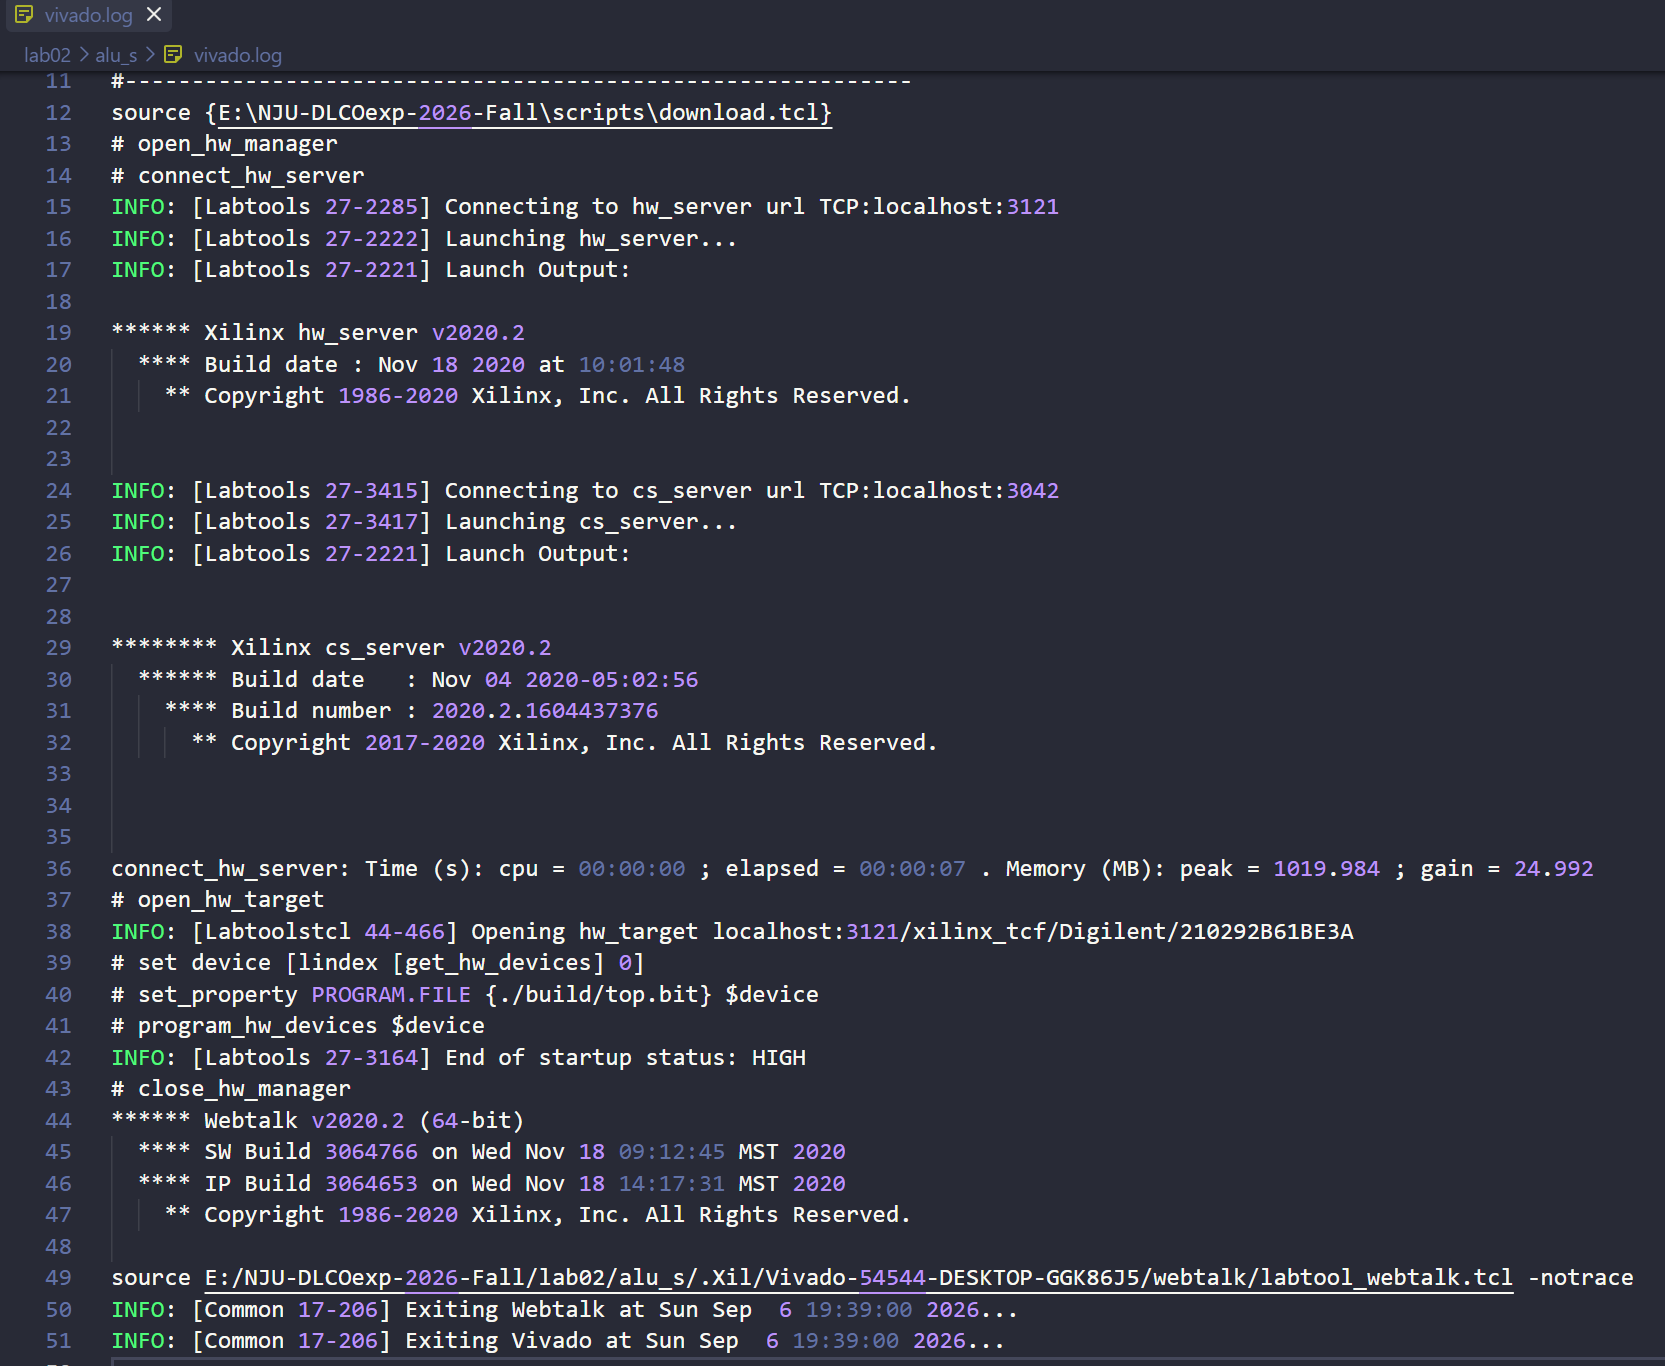
\includegraphics[width=0.7\textwidth]{lab02_build.png}
%     \caption{Vivado 综合与实现完成}
% \end{figure}

\section{测试方法}
验证从两方面进行：一是用 Vivado 做功能仿真观察波形并自动比对，二是下载到开发板实测；不依赖课程 OJ 判题。

\textbf{仿真（自校验）}：\texttt{tb.v} 内置一个独立的参考模型，用 5 位运算对每种操作数组合重算期望的 $F$/标志，再与 DUT 输出逐项比对，不一致即打印 \texttt{MISMATCH} 并累计错误，从而避免``以 DUT 验证 DUT''。测试信号的选择上，操作数取 5 个代表性值——全零（0，触发 \texttt{zero}）、\texttt{+1}（触发进位/借位）、最大正数 \texttt{+7}、最小负数 \texttt{-8}（补码边界）与全 1（\texttt{-1}，借位/比较边界），两两组合共 $5\times5$ 组，每组遍历 8 种运算，合计 200 组输入全部自动比对。

\textbf{上板实测}：$A$=拨码 \texttt{SW[10:7]}，$B$=\texttt{SW[6:3]}，运算选择 \texttt{ALUctr}=\texttt{SW[2:0]}。\texttt{SW[2:0]} 依次置 000--111 对应表~\ref{tab:alu} 的 8 种运算，拨入若干组 $A$/$B$，观察 \texttt{LED[10:7]}（$F$ 二进制）、\texttt{LED[0]}/\texttt{LED[1]}/\texttt{LED[2]}（\texttt{cf}/\texttt{zero}/\texttt{of}）与最右一位数码管显示的数值，重点核对加减法的进位/借位、负数显示与溢出标志。

\section{实验结果}

\subsection{仿真结果}
运行 \texttt{sim.bat}，testbench 对 200 组输入全部自动比对通过，Vivado 日志输出：
\begin{verbatim}
[PASS] all 200 vectors OK.
\end{verbatim}
波形上逐组验证：\texttt{ALUctr}=000/001 时加法/减法结果与 \texttt{cf}（进位/借位）正确；\texttt{zero} 在结果全零时拉高；对有符号溢出的组合（如 $7+1$、$-8-1$）\texttt{of} 正确置 1；010--111 各逻辑/比较运算输出与真值一致。

% TODO 2/3：截 Vivado 波形图（含 A/B/ALUctr/F/cf/zero/of），存为 figures/lab02_wave.png，取消下面注释
% \begin{figure}[htbp]
%     \centering
%     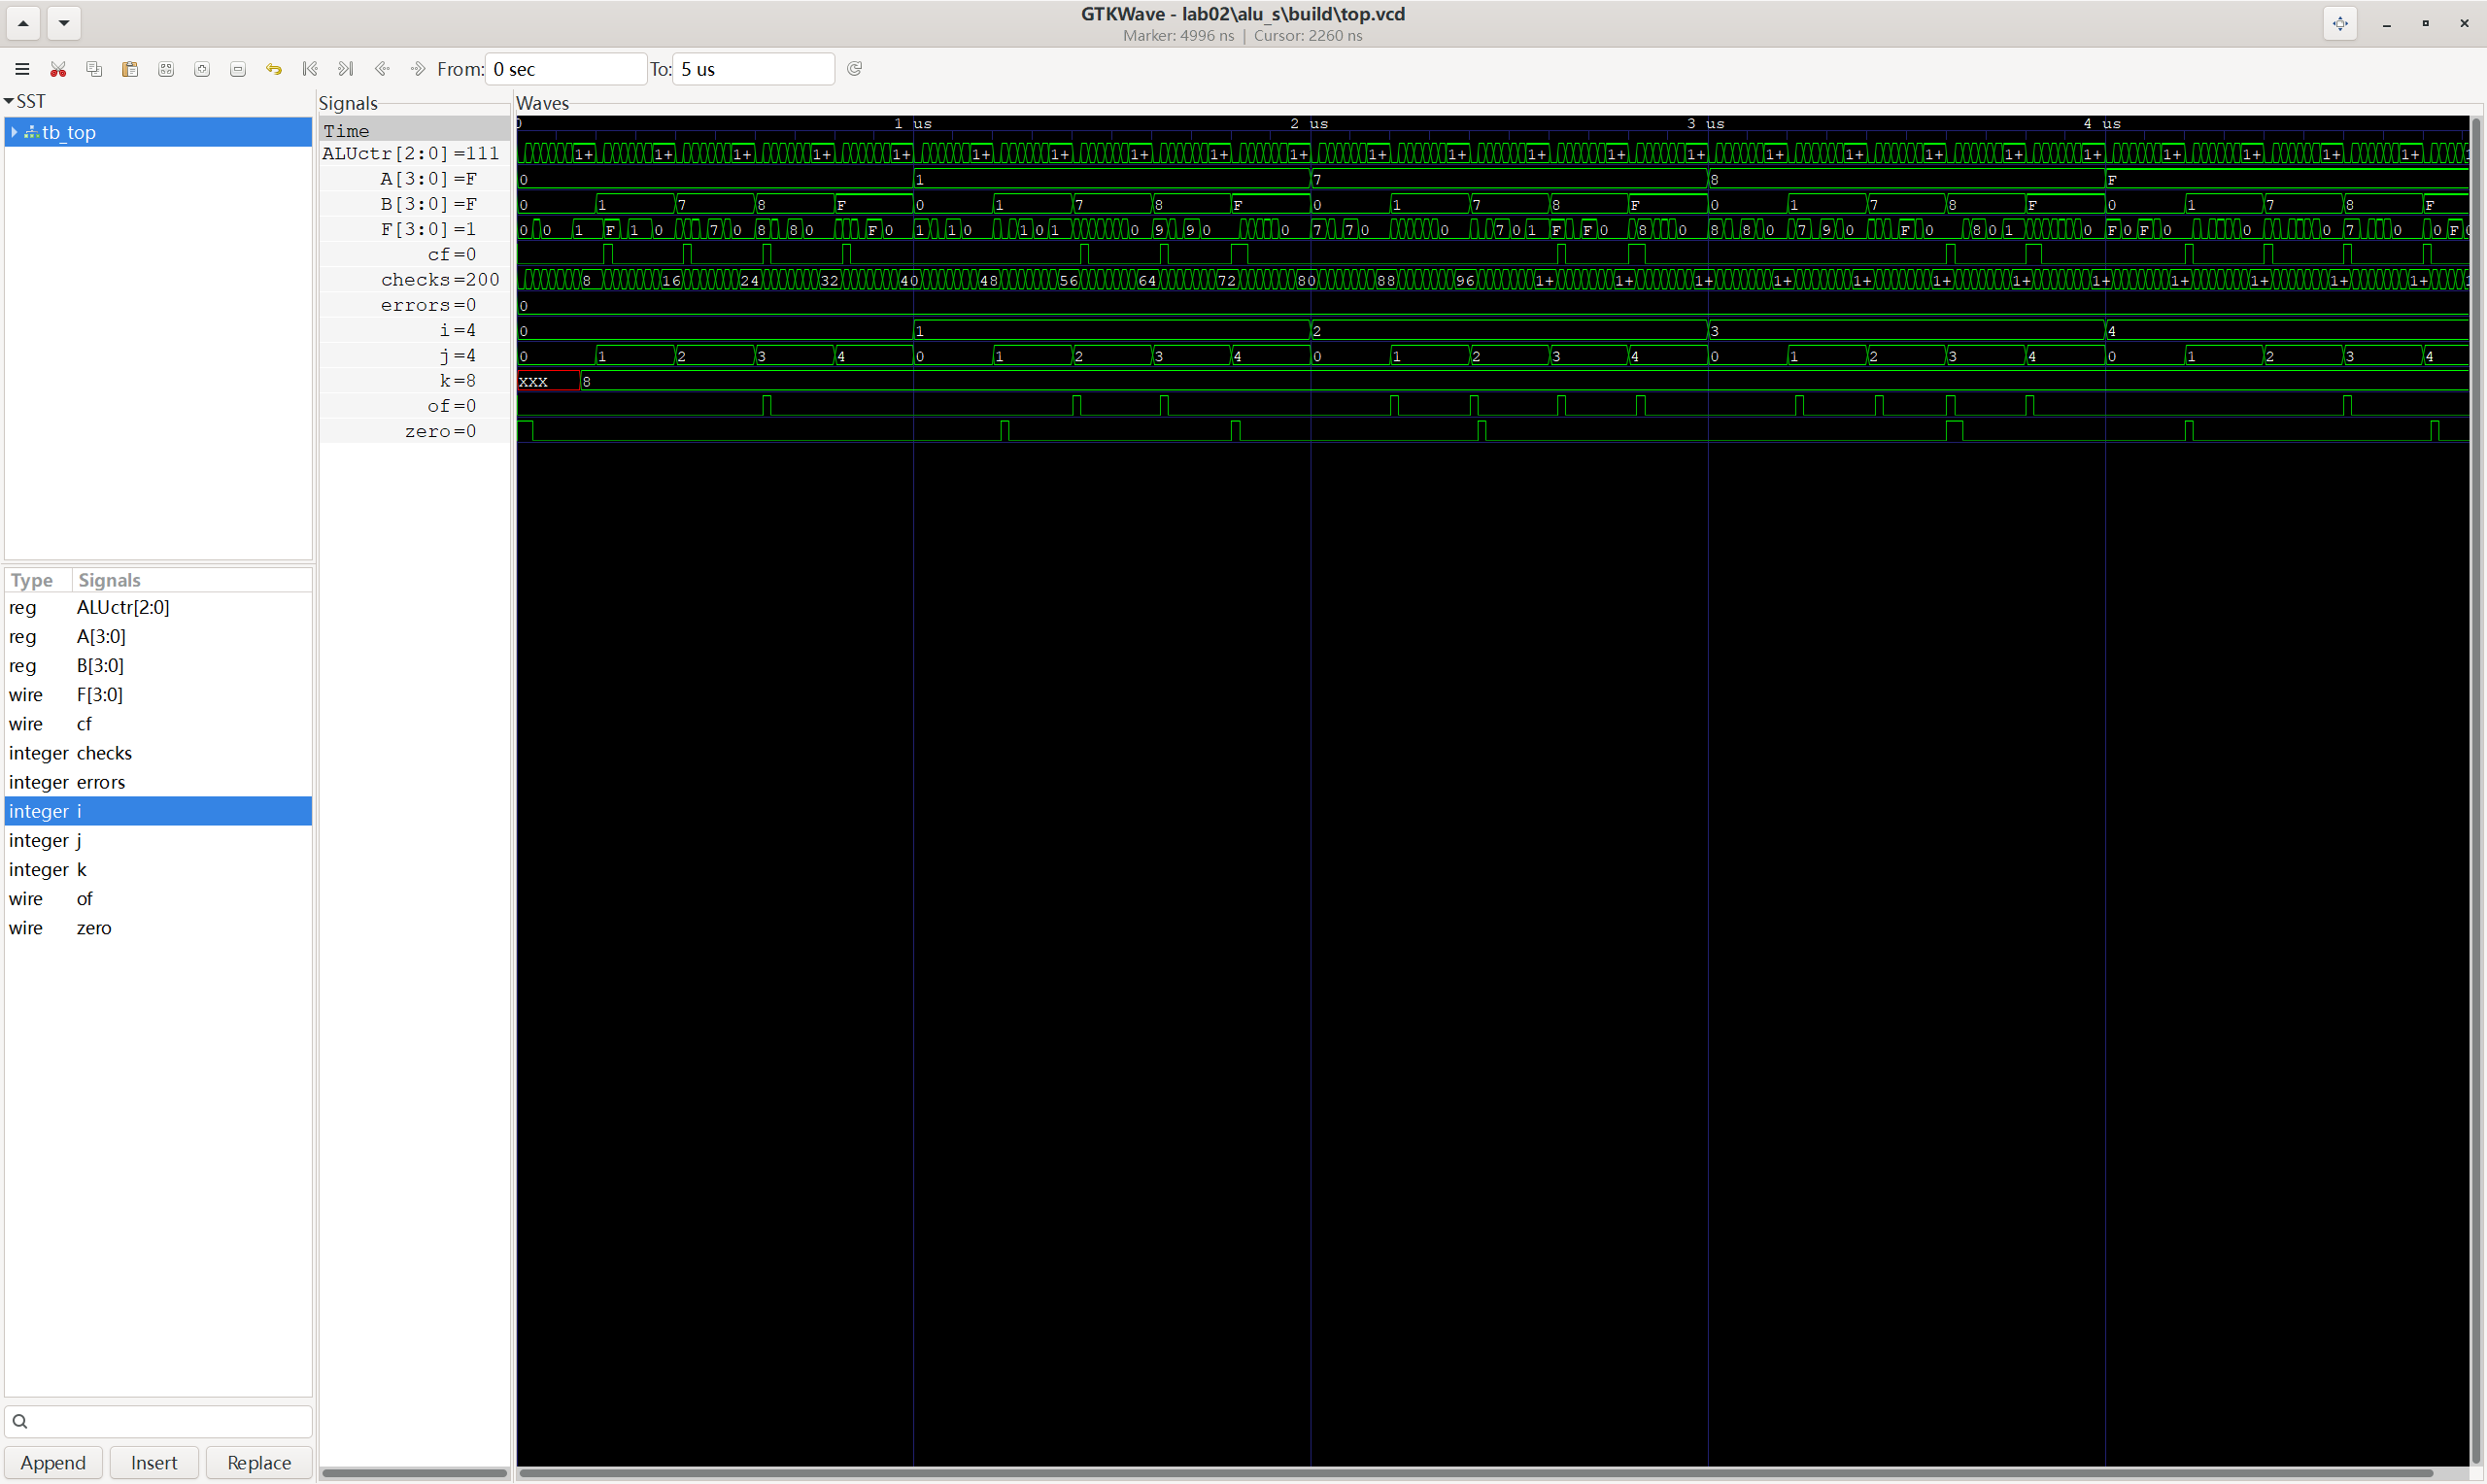
\includegraphics[width=0.9\textwidth]{lab02_wave.png}
%     \caption{ALU 功能仿真波形}
% \end{figure}

\subsection{上板结果}
下载比特流后实测（\texttt{ALUctr} 由 \texttt{SW[2:0]} 给定，\texttt{SW[2:0]}=000/001/011 分别为加/减/与）：
\begin{itemize}
    \item 加法 $A=2,B=3$：$F=5$，\texttt{LED[10:7]}=0101，\texttt{cf}/\texttt{zero}/\texttt{of} 均熄灭，数码管显示 5；
    \item 加法 $A=7,B=1$：$F=1000$（已超出补码范围 +7，\texttt{of} 应置 1），\texttt{LED[2]} 点亮，数码管显示 8；
    \item 减法 $A=3,B=5$：$F=1110$（$-2$），\texttt{LED[0]}（借位）点亮，数码管显示负数绝对值 2；
    \item 与运算 $A=7,B=5$：$F=0101$，\texttt{LED[10:7]}=0101，三个标志熄灭，数码管显示 5。
\end{itemize}
现象与仿真及表~\ref{tab:alu} 真值一致（若 $|F|>9$，数码管超出 0--9 译码范围会熄灭，此时以 \texttt{LED} 二进制为准）。

% TODO 3/3：贴上板实测照片（可选），存为 figures/lab02_board.jpg，取消下面注释
% \begin{figure}[htbp]
%     \centering
%     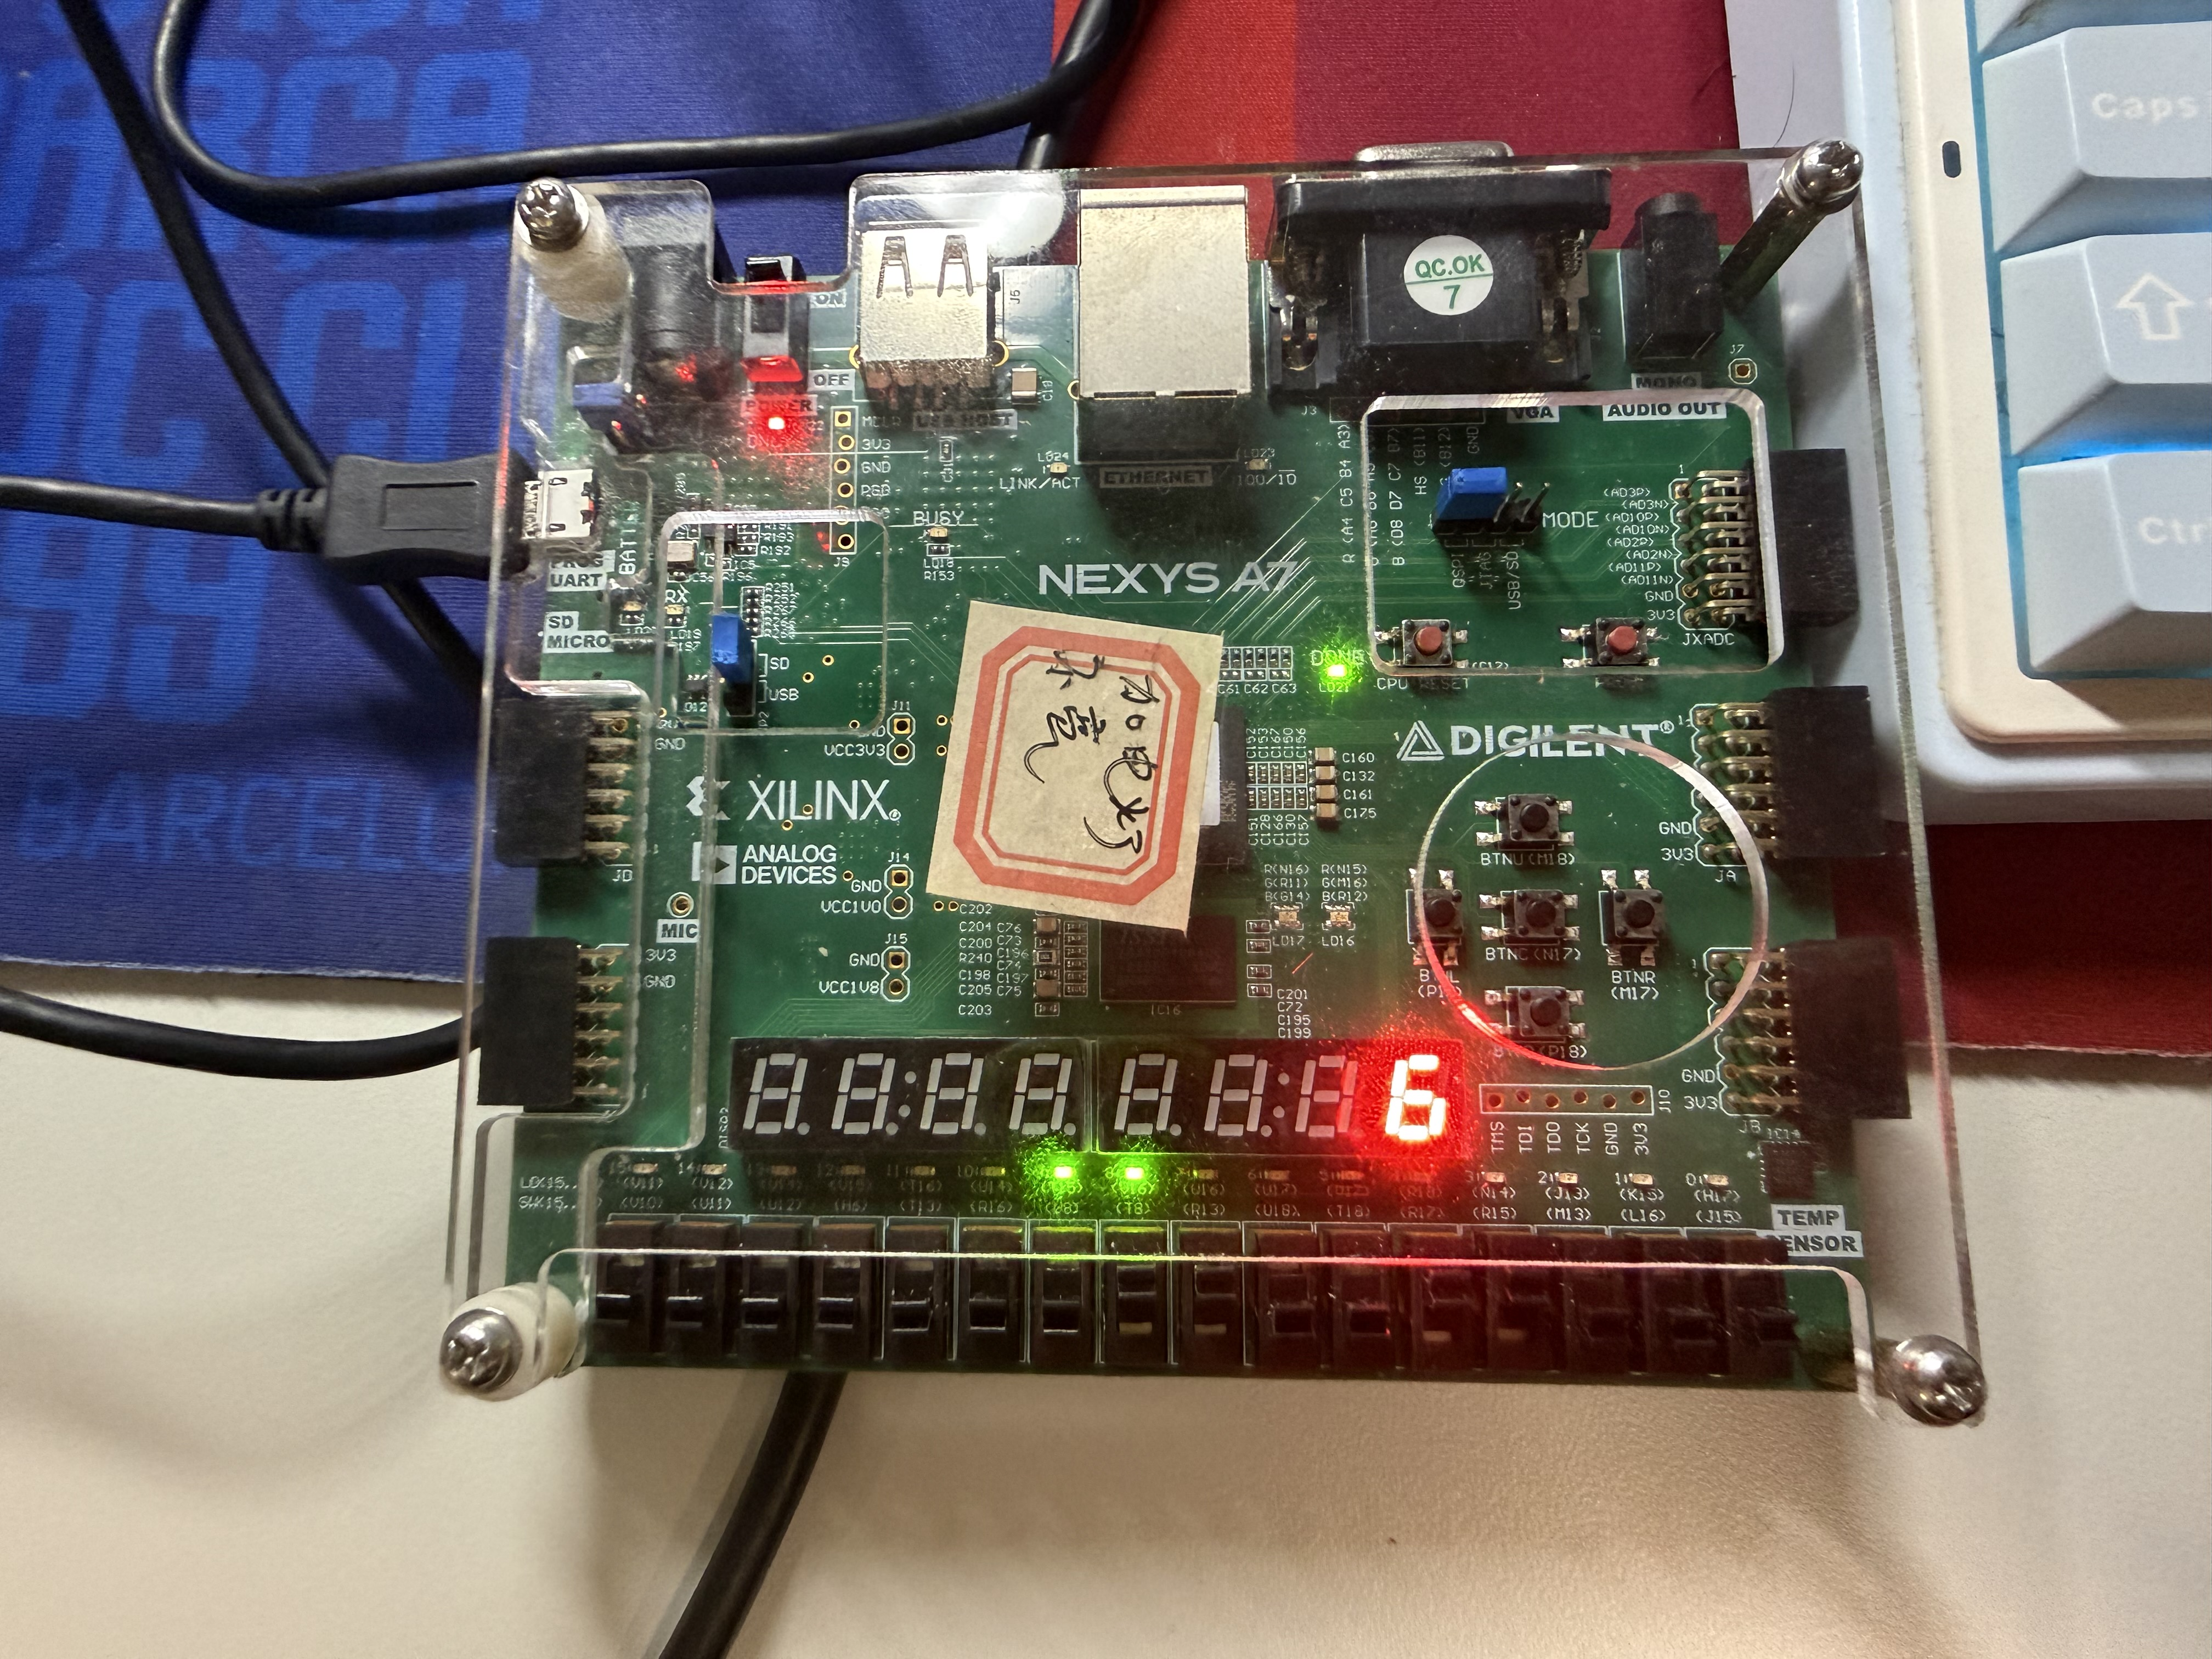
\includegraphics[width=0.6\textwidth]{lab02_board.jpg}
%     \caption{ALU 上板实测照片}
% \end{figure}

\section{问题与解决办法}
\begin{itemize}
    \item \textbf{标志信号残留}：\texttt{casez} 各分支若只对 $F$ 赋值，前一次加/减遗留的 \texttt{cf}/\texttt{zero}/\texttt{of} 会串到随后的逻辑运算结果上。解决：在 \texttt{always} 块开头对 $F$ 与三个标志统一清零，算术分支再按需赋值。
    \item \textbf{有符号小于需按补码解释}：直接写 $A<B$ 会把操作数当无符号数比较。解决：比较前用 \$signed() 把 4 位输入按二进制补码解释，再比较。
    \item \textbf{单位数码管如何显示符号/多位结果}：七段数码管只有一位且 \texttt{bcd7seg} 仅译 0--9，无法直接显示负号和十六进制结果。解决：\texttt{top.v} 中对负数求补码绝对值、显示数值大小，符号位由 \texttt{LED[10:7]} 的 $F[3]$ 判读，结果超出 0--9 时以 LED 二进制为准。
\end{itemize}

\section{启示与建议}

\textbf{启示：}
\begin{enumerate}
    \item 熟练掌握 \texttt{casez}/\texttt{always @(*)} 描述多功能组合电路，以及 ``先清零后按分支赋值'' 避免状态残留的写法。
    \item 理解了无符号进位（\texttt{cf}）与有符号溢出（\texttt{of}）是两套判据：前者看第 5 位，后者看操作数与结果的符号位，不能混用。
    \item 自校验 testbench 用独立参考模型自动比对 200 组向量，比人工逐个看波形更可靠、可回归。
\end{enumerate}

\textbf{建议：} 单位数码管难以完整显示 4 位十六进制结果与符号。后续可改用 8 位数码管扫描显示、增加减法标志（是否负）提示位，让上板读数更直观。

\end{document}
